\documentclass[12pt, legalpaper, twocolumn]{article}
% 10pt es el tamaño de letra por default
% para modificarlo desde documentclass, solo permite 10pt, 11pt y 12. 
% Prueba comentario
\usepackage{graphicx} % Required for inserting images
\usepackage{float} % Se utiliza para el posicionamiento forzado de los elementos del documento (figuras y tablas)
\usepackage{subcaption} %mozaico de figuras
\usepackage{pdflscape}


\usepackage[table,xcdraw]{xcolor} %para añadir color a las celdas de una tabla
\usepackage[normalem]{ulem} %para subrayar texto y generar otro tipo de subrayado
\useunder{\uline}{\ul}{}


\usepackage{enumitem} %generar listas con símbolos
\usepackage{pifont} %permite modificar los símbolos de las listas

\renewcommand{\labelitemii}{$ ? $} %para cambiar el símbolo por cuenta del usuario, este debe estar entre los sísmbolos de pesos. En este caso, se añade doble guión medio.
%labelitemi, al añadir otra "i" se indica el nivel de la tabla enumerada en el que se va a colocar el símbolo .

\usepackage{parskip} %para quitar sangría
\setlength{\parskip}{2mm}

\usepackage{blindtext} %texto aleatorio

\usepackage[spanish,mexico]{babel} %definimos el idioma español, para México.


\usepackage{xcolor} % ES EL PAQUETE PARA AÑADIR COLOR AL TEXTO HTML, RGB, ESCALA DE GRISES.

\definecolor{miguel}{RGB}{13,20,219}

\definecolor{color2}{cmyk}{0.5,.1,0.7,0.1}

\definecolor{color3}{gray}{0.6}

\definecolor{bittersweet}{rgb}{1.0, 0.44, 0.37}

\definecolor{color4}{HTML}{915C83}


\colorlet{color5}{magenta!50!green}


\usepackage{ragged2e}

\usepackage{multicol}

\title{\Huge{Tiro con arco}}
\author{\small{Miguel Carrillo}}
\date{30 de Enero 2025}


\begin{document}

\maketitle

\begin{abstract}
    En este documento se explica en qué consiste el tiro con arco, se mencionan los accesorios necesarios para practicar este deporte y se detallan las reglas que rigen esta actividad.
\end{abstract}

\section{\LARGE{Introducción}}

Elaboración de mi \textbf{primer} \emph{documento} para visualizar las opciones del tipo de \texttt{documento}. 

El tiro con \huge{arco} es un deporte en el que los participantes disparan flechas usando un arco con el objetivo de alcanzar una diana o blanco lo más cerca posible del centro. La \large{precisión} es clave, y cada disparo es puntuado según la cercanía al centro de la diana. En la figura \ref{tiro1}, se muestra una foto de un competidor.

\begin{figure}[H]
    \centering
    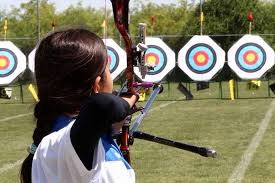
\includegraphics[scale=1]{tiro_arco.jpg} 
    \caption{Imagen ilustrativa del tiro con arco.}
    \label{tiro1}
\end{figure}

El tiro con arco es una práctica 'antigua' que comenzó como una técnica de caza y en la guerra. Sin embargo, como deporte organizado.
Corea del Sur domina este deporte a nivel olímpico. Han ganado más de 40 medallas (incluyendo alrededor de 27 de oro) desde que se reintrodujo en 1972. El éxito de Corea del Sur se atribuye a su sistema de entrenamiento riguroso y a la enorme popularidad del deporte en el país. 
%La probabilidad de que ganen los jefes de Kansas City es del 50\%.

\section{Mozaico de figuras}

A continuación se muestran los accesorios del tiro con arco. Por ejemplo, en la figura \ref{a} son las flechas y en la figura \ref{b} se observa la diana

\begin{figure}[H] % primeras dos subfiguras
    \begin{subfigure}{0.45\textwidth}
        \centering
        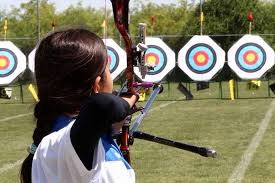
\includegraphics[scale=1]{tiro_arco.jpg} 
        \caption{Flechas}
        \label{a}
    \end{subfigure}
    \begin{subfigure}{0.45\textwidth}
        \centering
        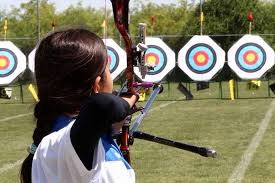
\includegraphics[scale=1]{tiro_arco.jpg} 
        \caption{Soporte}
        \label{b}
    \end{subfigure} 
    
    \begin{subfigure}{0.45\textwidth} % otras dos subfigura
        \centering
        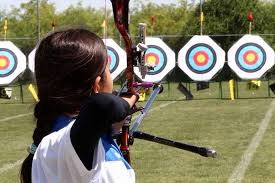
\includegraphics[scale=1]{tiro_arco.jpg} 
        \caption{Visor}
        \label{c}
    \end{subfigure}
    \begin{subfigure}{0.45\textwidth}
        \centering
        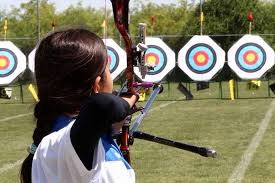
\includegraphics[scale=1]{tiro_arco.jpg} 
        \caption{Arco}
        \label{c}
    \end{subfigure}
    \caption{Accesorios del tiro con arco.}
\end{figure}

\subsection{Más figuras}

\newpage

\begin{landscape}
    \begin{figure}[H]
        \centering
        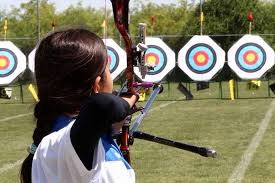
\includegraphics[scale=1]{tiro_arco.jpg} 
        \caption{Figura más grande}
        \label{fig:enter-label}
    \end{figure}
\end{landscape}

\newpage

\section{Países ganadores en tiro con arco}

A continuación se muestra la tabla \ref{tab1} de ganadores de medalla de oro en tiro con arco desde 1900:

\begin{table}[H]
    \centering
    \begin{tabular}{|c|c|}
    \hline
      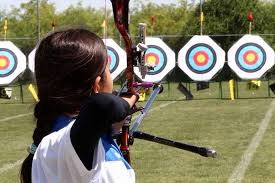
\includegraphics[scale=1]{tiro_arco.jpg}     &  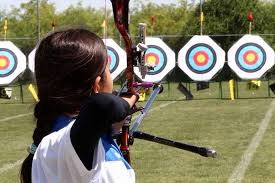
\includegraphics[scale=1]{tiro_arco.jpg}   \\
      \hline
      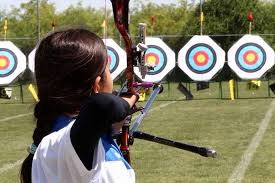
\includegraphics[scale=1]{tiro_arco.jpg}    & 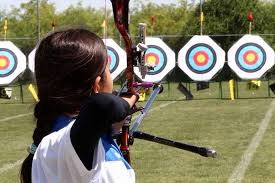
\includegraphics[scale=1]{tiro_arco.jpg} 
    \end{tabular}
    \caption{Caption}
    \label{tab:my_label}
\end{table}





\begin{table}[H]
    \centering
    \begin{tabular}{c|c|c}
      Países   &  Cantidad de medallas & Part. en juegos olimp.\\
      México   &            10         & 20\\
      Corea del sur &       9          &  30\\
      China         &       8          & 10
    \end{tabular}
    \caption{Tabla histórica de medallas en tiro con arco.}
    \label{tab1}
\end{table}

%\noindent
Otra forma de generar o modificar la tabla 1 es con el generador de tablas en línea. De esta forma, podemos obtener la tabla \ref{tab2}


\begin{table}[H]
\begin{tabular}{|c|c|c|}
\hline
\rowcolor[HTML]{67FD9A} 
{\color[HTML]{333333} \textbf{Países}} & {\color[HTML]{333333} \textbf{Cantidad de medallas}} & {\color[HTML]{333333} \textbf{Participación en juegos olimpicos}} \\ \hline
\rowcolor[HTML]{FFFFFF} 
{\color[HTML]{333333} {\ul México}}           & {\color[HTML]{333333} 20} & {\color[HTML]{333333} {\ul 25}} \\ \hline
\rowcolor[HTML]{FFFFFF} 
{\color[HTML]{333333} \textit{Corea del Sur}} & {\color[HTML]{333333} 10} & {\color[HTML]{333333} 25}       \\ \hline
\rowcolor[HTML]{FFFFFF} 
China                                         & 5                         & 25                              \\ \hline
\end{tabular}
\caption{Nueva tabla.}
\label{tab2}
\end{table}



A continuación vamos a generar una lista no enumerada. \underline{Enlistemos} los accesorios para practicar tiro con arco

\begin{itemize}  % representa el primer nivel de la lista no enumerada
    \item[\ding{36}] Flechas
        \begin{itemize} %segundo nivel de lista no enumerada
            \item[\ding{116}] Material 1
            \item Material 2
        \end{itemize}
    \item[\ding{61}] \textcolor{color5}{Arco}
        \begin{itemize} %segundo nivel de lista no enumerado
            \item Compuesto
                \begin{itemize} %tercer nivel de lista no enumerada
                    \item Simple
                \end{itemize}
        \end{itemize}
    \item [\ding{61}]Soporte para flechas
    \item[\ding{61}] Pechera
    \item 
\end{itemize}

Aquí se muestra una lista enumerada.

\begin{enumerate}
    \item \textcolor{color4}{\uline{\textbf{México}}}
        \begin{enumerate}
            \item Categoría olímpica.
        \end{enumerate}
    \item China
    \item Corea del Sur
    \item \textcolor{bittersweet}{Países Bajos}
\end{enumerate}

\section{Reglas del tiro con arco}

\begin{flushright}

Vamos a desglozar las \uline{reglas} del juego para competencia a nivel \uuline{olímpico}. Nos basaremos en el \textcolor{magenta}{reglamento} del Comité \uwave{Olímpico}   \textcolor{miguel}{Internacional}. Ahora probemos con otros \textcolor{color2}{colores}. Probemos con escala de \textcolor{color3}{grises.} 
\end{flushright}

\begin{flushleft}
\blindtext
\end{flushleft}

\begin{center}
    
Vamos a desglozar las \uline{reglas} del juego para competencia a nivel \uuline{olímpico}. Nos basaremos en el \textcolor{magenta}{reglamento} del Comité \uwave{Olímpico}   \textcolor{miguel}{Internacional}. Ahora probemos con otros \textcolor{color2}{colores}. Probemos con escala de \textcolor{color3}{grises.} 
\end{center}


\newpage

%\begin{multicols}{2}
Es imposible situar los inicios de la arquería en una fecha precisa. Tal fecha, aun de conocerse, solo podría valer para una zona geográfica en concreto. No obstante, se acuerda que la práctica se remonta a la invención de sus dos elementos principales: el arco y la flecha. Las puntas de flecha más antiguas, descubiertas en la cueva de Sibudu en Sudáfrica, datan de hace aproximadamente 64 000 años,2 aunque estas flechas primitivas podrían no haber sido propulsadas por arcos sino por el átlatl. Por su parte, la primera prueba segura de arcos en Europa, proveniente de pinturas rupestres en las cuevas de Valltorta y Morella en España, data del paleolítico tardío, alrededor de hace 40 000 años. Sin embargo, no se tiene constancia segura de cómo ni cuándo se inventó el arco.3 La aparición del tiro con arco revolucionó en un principio la caza durante la prehistoria.

\begin{figure}[H]
    \centering
    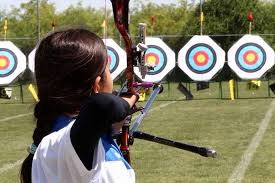
\includegraphics[scale=1]{tiro_arco.jpg} 
    \caption{Figura}
    \label{fig:enter-label}
\end{figure}

Ya en la era antigua, las primeras civilizaciones le dieron al arco un propósito bélico.

En la civilización clásica, en especial entre los persas, macedonios, nubios, griegos, partos, indios, japoneses, chinos y coreanos, se recurría a un gran número de arqueros en sus ejércitos. Las flechas eran especialmente destructivas contra formaciones cerradas, y el uso de flechas era, muchas veces, decisivo.

Durante la Edad Media, el tiro con arco en la guerra no fue tan decisivo y dominante en Europa Occidental. Los arqueros eran los soldados peor pagados en el ejército o eran reclutados del campesinado. Esto era debido a que el arco y la flecha eran mucho más baratos que el equipo de un hombre de armas con una buena armadura y una espada. Los arqueros profesionales requerían un largo entrenamiento y caros arcos para ser efectivos, así que era bastante raro verlos en Europa (véase arco largo inglés).

Sin embargo, el tiro con arco tuvo un desarrollo importante en Asia y el mundo islámico. Los arqueros a caballo fueron una de las principales fuerzas militares del ejército de Genghis Khan. En los tiempos modernos aún se sigue practicando en algunos países asiáticos, pero no a nivel de competición internacional. Ciertos pueblos de Asia Central fueron especialmente habilidosos en el tiro con arco a caballo siendo deporte nacional en el reino de Bután, Corea del Sur y Mongolia.


%\end{multicols}

\end{document}